\documentclass[11pt,a4paper]{article}

\newcommand{\tumsoTime}{13:00 น. - 16:00 น.}
\newcommand{\tumsoRound}{2}

\usepackage{../style/tumso}

\begin{document}

\begin{problem}{Autocomplete}{standard input}{standard output}{1 second}{256 megabytes}{100}

  ภาษา TUMSO (The Untyped Microlanguage without Strings and Objects) เป็นภาษาที่ใช้สำหรับการคำนวณจำนวนเต็ม

  \subsection*{ภาษา TUMSO}

  ไวยากรณ์ของภาษา TUMSO มีดังนี้ (ให้อ่าน \texttt{::=}  ว่า "คือ" และอ่าน \texttt{|} ว่า "หรือ")

  \begin{codetumso}[frame=single]
<program> ::= <expression>

<expression> ::= <number>
               | TRUE
               | FALSE
               | <identifier>
               | (CALL <expression> <expression>)
               | (FUNCTION (<identifier>) <expression>)
               | (LET <identifier> = <expression> IN <expression>)
               | (IF <expression> THEN <expression> ELSE <expression>)
               | (PLUS <expression> <expression>)
               | (MINUS <expression> <expression>)
               | (IS_EQUAL <expression> <expression>)
  \end{codetumso}

  \begin{itemize}
    \item \texttt{<number>} เป็นจำนวนเต็ม ตัวอย่างเช่น \texttt{-1234}
    \item \texttt{<identifier>} เป็นชื่อตัวแปร ประกอบไปด้วยอักขระในช่วง \texttt{a} ถึง \texttt{z} และเครื่องหมาย \texttt{\_} เช่น \texttt{the\_sum\_of\_two\_numbers}
  \end{itemize}

  โทเคนในภาษานี้ได้แก่ ตัวเลข \texttt{TRUE} \texttt{FALSE} \texttt{CALL} \texttt{FUNCTION} \texttt{LET} \texttt{=} \texttt{IN} \texttt{IF} \texttt{THEN} \texttt{ELSE} \texttt{PLUS} \texttt{MINUS} \texttt{IS\_EQUAL} และตัวแปร โดยโทเคนจะต้องถูกแยกออกจากกันด้วยช่องว่าง วงเล็บ หรืออักขระขึ้นบรรทัด

  \pagebreak

  \subsection*{ความหมายของโครงสร้างทางภาษา}

  \begin{itemize}
    \item สำหรับตัวเลข และ \texttt{TRUE} กับ \texttt{FALSE} จะได้ค่าผลลัพธ์เป็นเป็นค่าตัวเลข ค่า \texttt{TRUE} หรือค่า \texttt{FALSE} นั้น ๆ
    \item สำหรับตัวแปร จะได้ค่าผลลัพธ์เป็นค่าที่ตัวแปรนั้นเก็บอยู่
    \item สำหรับ \texttt{(CALL <f> <a>)} ค่าผลลัพธ์ของ \texttt{<f>} ควรจะเป็นค่าฟังก์ชัน และจะได้ค่าผลลัพธ์เป็นค่าของการเรียกใช้ฟังก์ชันนั้นด้วยพารามิเตอร์ซึ่งก็คือค่าผลลัพธ์ของ \texttt{<a>}
    \item สำหรับ \texttt{(FUNCTION (<a>) <e>)} จะได้ค่าผลลัพธ์เป็นค่าฟังก์ชันนั้น ๆ ที่มีพารามิเตอร์คือ \texttt{<a>} และเมื่อมีการเรียกฟังก์ชันด้วยพารามิเตอร์ \texttt{<v>} จะสร้างตัวแปร \texttt{<a>} ขึ้นมาเก็บค่า \texttt{<v>} และได้ค่าผลลัพธ์เป็น \texttt{<e>} (โดยที่ \texttt{<a>} สามารถถูกอ้างถึงได้ใน \texttt{<e>})
    \item สำหรับ \texttt{(LET <x> = <v> IN <e>)} จะสร้างตัวแปร \texttt{<x>} ขึ้นมาเก็บค่าของ \texttt{<v>} และได้ค่าผลลัพธ์เป็น \texttt{<e>} (โดยที่ \texttt{<x>} สามารถถูกอ้างถึงได้ในทั้ง \texttt{<v>} และ \texttt{<e>})
    \item สำหรับ \texttt{(IF <cond> THEN <then> ELSE <else>)} หาก \texttt{<cond>} มีค่าคือผลลัพธ์คือ \texttt{TRUE} จะได้ค่าผลลัพธ์เป็น \texttt{<then>} แต่หาก \texttt{<cond>} มีค่าคือผลลัพธ์คือ \texttt{FALSE} จะได้ค่าผลลัพธ์เป็น \texttt{<else>}
    \item สำหรับ \texttt{(PLUS <a> <b>)} ค่าผลลัพธ์ของ \texttt{<a>} และ \texttt{<b>} ควรจะเป็นตัวเลข และจะได้ค่าผลลัพธ์เป็น \texttt{<a>}~$+$~\texttt{<b>}
    \item สำหรับ \texttt{(MINUS <a> <b>)} ค่าผลลัพธ์ของ \texttt{<a>} และ \texttt{<b>} ควรจะเป็นตัวเลข และจะได้ค่าผลลัพธ์เป็น \texttt{<a>}~$−$~\texttt{<b>}
    \item สำหรับ \texttt{(IS\_EQUAL <a> <b>)} ค่าผลลัพธ์ของ \texttt{<a>} และ \texttt{<b>} ควรจะเป็นตัวเลข และจะได้ค่าผลลัพธ์เป็น \texttt{TRUE} หาก \texttt{<a>}~$=$~\texttt{<b>} และจะได้ค่าผลลัพธ์เป็น \texttt{FALSE} หาก \texttt{<a>}~$\ne$~\texttt{<b>}
  \end{itemize}

  \subsection*{ตัวอย่างโปรแกรมในภาษา TUMSO}

  \begin{tabular}{|M{12cm}|M{3.5cm}|N}
    \hline
    \textbf{โปรแกรม} & \textbf{ผลลัพธ์} & \\[5pt]
    \hline \hline

%%%%%%%%%%%%%%%%%%%%%%%%%%%%%%%%%%%%%%%%%%%%%%%%%%%%%%%%%%%%%%%%%%%%%%%%%%%%%%%%

    {\begin{codetumso}
FALSE
    \end{codetumso}} & {\begin{codetumso}
FALSE
    \end{codetumso}}
    \\ \hline

%%%%%%%%%%%%%%%%%%%%%%%%%%%%%%%%%%%%%%%%%%%%%%%%%%%%%%%%%%%%%%%%%%%%%%%%%%%%%%%%

    {\begin{codetumso}
(LET a = 1 IN
  (PLUS
    (LET a = 2 IN a)
    a))
    \end{codetumso}} & {\begin{codetumso}
3
    \end{codetumso}}
    \\ \hline

%%%%%%%%%%%%%%%%%%%%%%%%%%%%%%%%%%%%%%%%%%%%%%%%%%%%%%%%%%%%%%%%%%%%%%%%%%%%%%%%

    {\begin{codetumso}
(LET mult = (FUNCTION (a)
              (FUNCTION (b)
                (IF (IS_EQUAL 0 a)
                 THEN 0
                 ELSE (PLUS b (CALL (CALL mult b)
                                    (MINUS a 1)))))) IN
  (LET fact = (FUNCTION (n)
                (IF (IS_EQUAL 0 n)
                 THEN 1
                 ELSE (CALL (CALL mult n)
                            (CALL fact
                                  (MINUS n 1))))) IN
    (CALL fact 5)))
    \end{codetumso}} & {\begin{codetumso}
120
    \end{codetumso}}
    \\ \hline

%%%%%%%%%%%%%%%%%%%%%%%%%%%%%%%%%%%%%%%%%%%%%%%%%%%%%%%%%%%%%%%%%%%%%%%%%%%%%%%%

    {\begin{codetumso}
a
    \end{codetumso}} & {\begin{codetumso}
Error: `a' is undefined
    \end{codetumso}}
    \\ \hline

%%%%%%%%%%%%%%%%%%%%%%%%%%%%%%%%%%%%%%%%%%%%%%%%%%%%%%%%%%%%%%%%%%%%%%%%%%%%%%%%

    {\begin{codetumso}
(CALL 1 2)
    \end{codetumso}} & {\begin{codetumso}
Error: type mismatch
    \end{codetumso}}
    \\ \hline

  \end{tabular}

\section*{Task}

  ปัญหาการเรียกใช้ตัวแปรที่ไม่ได้ถูกนิยามไว้เป็นปัญหาที่พบได้ในภาษาโปรแกรมส่วนใหญ่ รวมถึงภาษา TUMSO ด้วย (ดูตัวอย่างโปรแกรมที่ 4 เป็นต้น) บาง IDE (Integrated development environment) เช่น Eclipse ของภาษา Java มีเครื่องมือแนะนำ\textit{ตัวแปรที่สามารถใช้ได้} ในตำแหน่งที่เคอร์เซอร์กำลังอยู่ เพื่อที่คุณจะได้ไม่เขียนโปรแกรมผิดตั้งแต่แรก

  \begin{figure}[h]
    \centering
    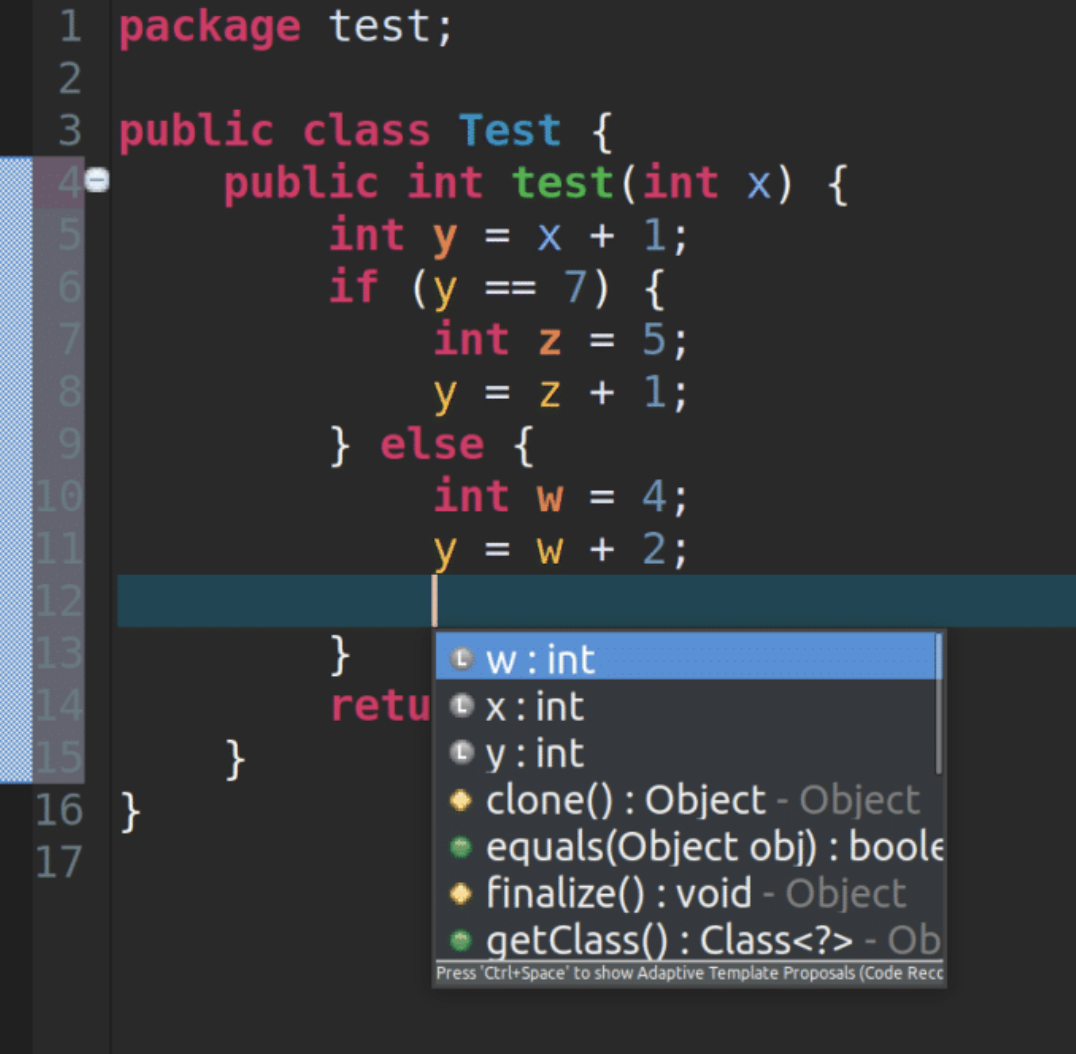
\includegraphics[width=0.6\textwidth]{calc-vars}
    \caption{ตัวอย่างโปรแกรม Eclipse ที่แนะนำตัวแปรที่สามารถใช้งานได้ในตำแหน่งที่เคอร์เซอร์อยู่สำหรับภาษา Java }
  \end{figure}

  หน้าที่ของคุณคือให้เขียนโปรแกรมรับโค้ดที่ไม่สมบูรณ์ในภาษา TUMSO โดยมีสัญลักษณ์ \texttt{\#} อยู่หนึ่งที่ในตำแหน่ง \texttt{<expression>} (แสดงถึงเคอร์เซอร์ในโปรแกรมที่กำลังเขียนอยู่) และแสดงผลตัวแปรทั้งหมดที่สามารถใช้ได้ที่ตำแหน่ง \texttt{\#}

\InputFile

  ประกอบไปด้วยโค้ดที่ไม่สมบูรณ์ในภาษา TUMSO ซึ่งมีอักขระ \texttt{\#} อยู่หนึ่งที่ในตำแหน่ง \texttt{<expression>} และหากแทนที่อักขระ \texttt{\#} ในโค้ดนี้ด้วย \texttt{<expression>} ใด ๆ (เช่น \texttt{0}) จะทำให้กลายเป็นโปรแกรมที่มีไวยากรณ์ถูกต้องในภาษา TUMSO โค้ดนี้จะมีความยาวกี่บรรทัดก็ได้

\OutputFile

  มี $n$ บรรทัด โดย $n$ คือจำนวนตัวแปรที่สามารถใช้ได้ในตำแหน่ง \texttt{\#} และแต่ละบรรทัดมีชื่อของตัวแปรที่สามารถใช้ได้ดังกล่าวในลำดับพจนานุกรม (lexicographic order)

\section*{Constraints}

  โค้ดที่ให้จะมีขนาดไม่เกิน $10^6$ ไบต์

\Examples

  \begin{tabular}{|M{12cm}|M{3.5cm}|N}
    \hline
    \textbf{ข้อมูลนำเข้า} & \textbf{ข้อมูลส่งออก} & \\[5pt]
    \hline \hline

%%%%%%%%%%%%%%%%%%%%%%%%%%%%%%%%%%%%%%%%%%%%%%%%%%%%%%%%%%%%%%%%%%%%%%%%%%%%%%%%

    {\begin{codetumso}
(LET mult = (FUNCTION (a)
              (FUNCTION (b)
                (IF (IS_EQUAL 0 a)
                 THEN 0
                 ELSE (PLUS b (CALL (CALL mult b)
                                    (MINUS a 1)))))) IN
  (LET fact = (FUNCTION (n)
                (IF (IS_EQUAL 0 n)
                 THEN 1
                 ELSE (CALL (CALL mult n)
                            (CALL fact
                                  (MINUS n 1))))) IN
    (CALL fact #)))
    \end{codetumso}} & {\begin{codetumso}
fact
mult
    \end{codetumso}}
    \\ \hline

%%%%%%%%%%%%%%%%%%%%%%%%%%%%%%%%%%%%%%%%%%%%%%%%%%%%%%%%%%%%%%%%%%%%%%%%%%%%%%%%

    {\begin{codetumso}
(IF TRUE THEN a ELSE (LET x = 1 IN #))
    \end{codetumso}} & {\begin{codetumso}
x
    \end{codetumso}} \\ \hline
\end{tabular}

\end{problem}

\end{document}
